\section{Linearized equations}\label{linear_problem}
To compute explicit solutions to the linear problem, 
we consider radially-localized axisymmetric disturbances of the form  
\begin{align}
  \delta f (r, z) = \delta f_1(r,z)\exp{(\ii k_x r)},
\end{align} 
%and similarly for $\dd P$ and $\dd\bm{v}$. 
where $k_x$ is a real wavenumber such that $|k_xr|\gg 1$, and the 
amplitude $\dd f_1(r,z)$ is 
a slowly-varying function of $r$. Then 
$\p_r\to i k_x$ when acting on the above primitive perturbations, and we may
neglect curvature terms. We take  
$k_x>0$ without loss of generality. Hereafter, we drop the subscript 1
on the amplitudes. 
%The frequency $\sigma = \omega +
%\ii s$ is generally complex, with $\omega$ being the real frequency
%and $s$ is the real growth rate. 

Introducing 
\begin{align}
  W \equiv \frac{\dd\rho}{\rho}, \quad Q \equiv \frac{\dd P}{\rho},
\end{align}
the linearized equations for 
locally isothermal dusty gas with the pressure
equation in place of the dust-fraction
(Eq. \ref{masseq}---\ref{momeq}, Eq. \ref{eff_energy}) are then:    

\begin{align}
  \ii\sigma W &= \ii k_x \dd v_r + \dd v_z^\prime +
  \dd v_r \p_r\ln{\rho} + \dd v_z\p_z\ln{\rho},\label{lin_mass}\\
  -\ii\sigma\dd v_r  &= 2\Omega\dd v_\phi 
% +  \delta\bm{F}\cdot\hat{\bm{r}}
- W F_r - \ii k_x Q,\label{lin_xmom}\\
  \ii\sigma\dd v_\phi &= \frac{\kappa^2}{2\Omega}\dd v_r + \frac{\p
    v_\phi}{\p z}\dd v_z, \label{lin_ymom}\\
  -\ii\sigma\dd v_z &= - W F_z - \left[Q^\prime + Q
    \left(\ln{\rho}\right)^\prime\right]  %\delta\bm{F}\cdot\hat{\bm{z}} 
,\label{lin_zmom}\\
  \ii\sigma Q &= \frac{P}{\rho}\left(\ii k_x \dd v_r + \dd
               v_z^\prime\right) + \frac{1}{\rho}\left(\dd v_r\p_rP + \dd v_z \p_zP\right)\notag\\
                &\phantom{=}-\frac{P}{\rho} \dd v_r\p_r
               \ln{c_s^2} %, \label{lin_energy} 
%+ \dd v_z \p_z\ln{c_s^2}\right),\label{lin_energy} 
               - \frac{\dd\mathcal{C}}{\rho},\label{lin_energy} 
\end{align}  
where $^\prime \equiv \p_z$ and recall $\bm{F} \equiv -\nabla P/\rho$. 
The linearized dust-duffusion function 
$\dd\mathcal{C}$ is given in  Appendix \ref{lin_dust}. 
% and $\dd\bm{F}$ is the linearized pressure
%force, given in Appendix \ref{lin_press}. 
Note that we have assumed a temperature profile that only depends on $r$.   

%; and 
%\begin{align}
%  \delta \bm{F} \equiv \frac{\dd\rho}{\rho^2}\nabla P -
%  \frac{1}{\rho}\nabla\dd P, 
%\end{align}
%$\dd\mathcal{C}$ is the linearized dust-duffusion function, given in
%Appendix \ref{lin_dust}. We consider stopping times appropriate for
%small grains in the Epstein regime. Note that for the axisymmetric
%problem, $\dd\bm{F}$ is purely meridional. 

Eq. \ref{lin_mass}---\ref{lin_energy} is a set of ordinary
differntial equations in $z$. All coefficients and amplitudes are
evaluated at a fiducial radius $r=r_0$, but their full $z$-dependence
is retained. We now discuss solutions to these equations in an unstratified disk 
 for the streaming instability (\S\ref{si}), and a stratified disk for the VSI (\S\ref{results}).  
 
 % Numerical solutions are generally required for the 
%vertically-stratified problem. 

\section{Dust-drag instabilities}\label{si}
In the special case of an unstratified disk (neglecting the vertical
component of the stellar gravity), we may also Fourier analyze in $z$
to obtain an algebraic dispersion relation of the form  
$\sum_{j=0}^{5}c_j(k_x,k_z)\sigma^j = 0$, where $k_z$ is a real
vertical wavenumber. The coefficients $c_j$ can be read 
off Eq. \ref{streaming_dispersion} in  Appendix \ref{compressible_streaming}. 
There we also show that this dispersion relation reduces to that for
the streaming instability (SI) in the limit of incompressible gas and small
$\tstop$ \citep{youdin05a,jacquet11}.   
 
\subsection{Overstable epicycles}
If we further consider the limit $k_z=0$, the incompressible dispersion
relation, Eq. \ref{streaming_incompressible}, reduces to 
\begin{align}      %streaming_incompressible
\ii \sigma^2 - \frac{\sigma}{\epsilon \tstop}  - \left(\ii \kappa^2 +
  \frac{k_xF_r}{\epsilon}\right) = 0. \label{kz_zero_si}
\end{align} 
%Here we use $\tau_\mathrm{s}=\tstop/(1-\tepsilon)$ for convenience. 
If the quadratic term is neglected, then $\imag{\sigma}<0$, implying
stability, as concluded by \cite{youdin05a}. 

However, retaining all the terms (but still in the incompressible
limit) can yield instability, as follows. Eq. \ref{kz_zero_si} admit
pure oscillations with $\sigma = -\omega$ when 
\begin{align*}
  \omega &= \pm \kappa, \\
  \tstop & = \frac{\omega}{ k _x F_r }
         \equiv t_{\mathrm{s}0}.
\end{align*} 
Since $\tstop\geq 0$, we require $k_xF_r > 0$ if $\omega = \kappa$;
and $k_xF_r < 0$ if $\omega = -\kappa$. For $k_x>0$ these marginally
stable epicycles require radial pressure gradients decreasing and increasing
outwards, respectively.  

%We require $\omega/k_xF_r> 0$  

We now perturb about this state of marginal stability by writing
$\sigma = \dd \sigma - \omega $ with $\dd\sigma = \ii\dd s -
\dd\omega$, $\tstop = t_{\mathrm{s}0} +
\dd\tstop $, and assume the $\dd$ quantities are small in
magnitude. Then 
\begin{align*} 
\dd s = \frac{2\epsilon \kappa^2 }{1 +
  4\epsilon^2 t_{\mathrm{s}0}^2\kappa^2}\dd \tstop. 
\end{align*}
Thus given $k_xF_r$, there exist growing modes 
when the stopping time is slightly larger than
$t_{\mathrm{s}0}$.  

%{\bf note: several approx used}

If we instead fix $\tstop$ and vary $k_xF_r$ about marginal stability,
a similar exercise yields  
\begin{align*} 
  \dd s = \frac{\epsilon \tstop^3}{1 +
  4\epsilon^2 \tstop^2 \kappa^2}\dd \left(k_x^2F_r^2\right).  
\end{align*}
Thus it is possible to destabilize the system by slightly increasing
$|k_xF_r|>\kappa/ \tstop$ (i.e. shorter radial wavelengths and/or
stronger pressure gradients).   


 
\citep[cf. the `convective overstability', ][]{klahr14,lyra14,latter16}.  




\subsection{Streaming instability}

{\bf note: kappa2 accounts for dust effect assuming smallh=0.05}

We now consider the streaming instability with $k_z\neq 0$. 
We solve Eq. \ref{streaming_dispersion} for selected cases where SI  
growth rates have been 
calculated analytically from full two-fluid disk models and measured 
from direct numerical particle-gas simulations 
\citep[namely][]{youdin07b,bai10b}. These authors use normalized
wavenumbers $K_{x,z} = \eta r k_{x,z}$ where
\begin{align} 
  \eta \equiv -\frac{1}{2\rhog r\OmK^2}\frac{\p P}{\p r} = 
  \frac{1}{2\left(1-\tepsilon\right)}\frac{F_r}{r\OmK^2}, 
\end{align} 
measures the pressure offset of Keplerian rotation. We use
$\eta=0.05c_s/r\OmK$. They also define the stopping time as
$\tau_\mathrm{s}=\tstop/(1-\tepsilon)$.  

Table \ref{si_compare} compares the eigenfrequencies obtained from the
one-fluid dispersion relation to that from the above studies. As  
expected eigenfrequencies agree better with decreasing $\tstop$ since
in that limit the mixture behaves more like a single fluid. Most 
importantly, we find the work done $\mathcal{W}>0$ in all cases, and
hence find growing oscillations. 

{\bf note: important to use largrangian pressure pert properly}
We also checked the growth rates $s$ satisfy 
\begin{align} 
  s = \frac{\left|\sigma\right|^2\imag\left(\Delta P
    \Delta\rho^*/\rho\right)}{2\real\left(\sigma\right)\rho\left(\left|\dd
  v_x\right|^2+\left|\dd
  v_z\right|^2\right)}, \label{si_check}
\end{align}
as implied by Eq. \ref{thermal_instability} and
Eq. \ref{pdv}. %, or directly from
%Eq. \ref{streaming_mass}---\ref{streaming_vz}. 
Interestingly, we find that for cases with
$\epsilon>1$, Eq. \ref{si_check} can be satisified with $\Delta
P\simeq \ii\dd v_x \p_rP/\sigma$, i.e. the radial pressure gradient
is responsible for growth. Conversely, for `linB' with $\epsilon
< 1$, one can approximate $\Delta P \simeq \dd P$ in Eq. \ref{si_check}. This
suggests that for SI in gas-dominated disks, the distinction between
Eulerian and Lagragian pressure perturbations is unimportant. 
{\bf but weak growth in this case}
%However
%in that case the gro 

In Table \ref{si_compare} we also calculate the phase difference
between the Lagragian pressure perturbation and density perturbations
as    
\begin{align*} 
\varphi \equiv -\sgn(\omega)\arg\left(\Delta P\Delta\rho^*\right)
        = \sgn(\omega)\arg\left(\Delta\rhog^*\Delta\rhod\right),\notag
\end{align*}
%where we have applied the isothermal equation of state for the second equality.
then $\varphi > 0 $ indicates pressure lagging behind density, which
is true for all the cases. In particular, `linB' indicates that growth
rates vanish as $\varphi \to 0$.  
Thus the streaming instability indeed stems  
from the gas pressure evolution lagging behind that of the dust 
density. 

%"generalized stokes number" would include other problem parameters,
%e.g. wavenumber  


{\bf suppose large scale pressure grad drops outwards. 
pert the sys by kicking more dust inwards. gas moves out, into region 
  of lower pressure in the bg. i.e. create pressure bump at larger
  radius. it attracts the first dust particles back out, plus some more
  because bump is larger. (move gas from higher density to lower
  density produce asymmetric bump/trough.}

\begin{deluxetable*}{llrrrrrr}
  \tablecolumns{8}
  \tablecaption{Selected eigenfrequencies for the streaming
    instability. \label{si_compare}
  }
  \tablehead{
    \colhead{Mode} & 
    \colhead{$\tau_\mathrm{s}\OmK$} &
    \colhead{$\epsilon$} &
     \colhead{$K_{x,z}$} &
      \colhead{$\sigma/\OmK$ (two-fluid)} &
    \colhead{$\sigma/\OmK$ (one-fluid)} &
    \colhead{$\mathcal{W}$ (arbitrary units)} &
      \colhead{$\Delta P$ lag}
  }
\startdata
 linA, \cite{youdin07b} &  $0.1$       & 3.0 & 30    & $-0.3480 +
 0.4190\ii$ & $0.3640 + 0.4249\ii$ & $0.90$ & $30\degr$\\ 

linB, \cite{youdin07b} & $0.1$        &  0.2 & 6 & $0.4999 +
0.0155\ii$&   $-0.4981 + 0.0054\ii$  & $1.54$ & $1.2\degr$ \\

linC,  \cite{bai10b}  & $10^{-2}$   &  2.0 & 1500&   $0.1049 +
0.5981\ii$   &  $0.1338 + 0.6650\ii$  & $0.15$& $11\degr$ \\

linD, \cite{bai10b} &  $10^{-3}$   &  2.0 & 2000 & $0.3225 + 
0.3154\ii$& $0.3219 + 0.3154\ii$ &  $1.28$ & $22\degr$ 
\enddata
\end{deluxetable*}


\subsection{Numerical example}

To demonstrate the above instabilities we numerically solve the
full dispersion relation, Eq. \ref{streaming_dispersion} at fixed $K_x
= 1500$ and $\epsilon=2$. Growth rates are shown in 
Fig. \ref{dusty_growth} as a function of $K_z$ at fixed $\taus\OmK=0.01$
(top panel, which includes `linC' in Table \ref{si_compare}); and as a
function of $\taus\OmK$ at fixed $K_z=50$ (bottom panel).   

The top panel shows that the streaming instability vanishes as
$K_z\to0$, but it dominates most of $K_z$
-space. The overstable epicycles become important for 
$K_z\lesssim 100$, but their growth rates are weak. We thus
expect streaming instabilities to dominate, provided small
lengthscales can be resolved. 

In the bottom panel we confirm that the overstable epicycles require a
sufficiently large stopping time at fixed wavenumbers. The vertical
dashed line is the critical stopping time 
\begin{align*}
  \tau_{\mathrm{s}0}\OmK = \frac{1}{2K_x\left(1-\tepsilon\right)^2} 
\end{align*}
in the above notation. For this example, $\tau_{\mathrm{s}0}\OmK\simeq
0.003$, as observed. On the other hand, the streaming instability
shows weak dependence on $\taus$ for this range of stopping times. 


\begin{figure}
  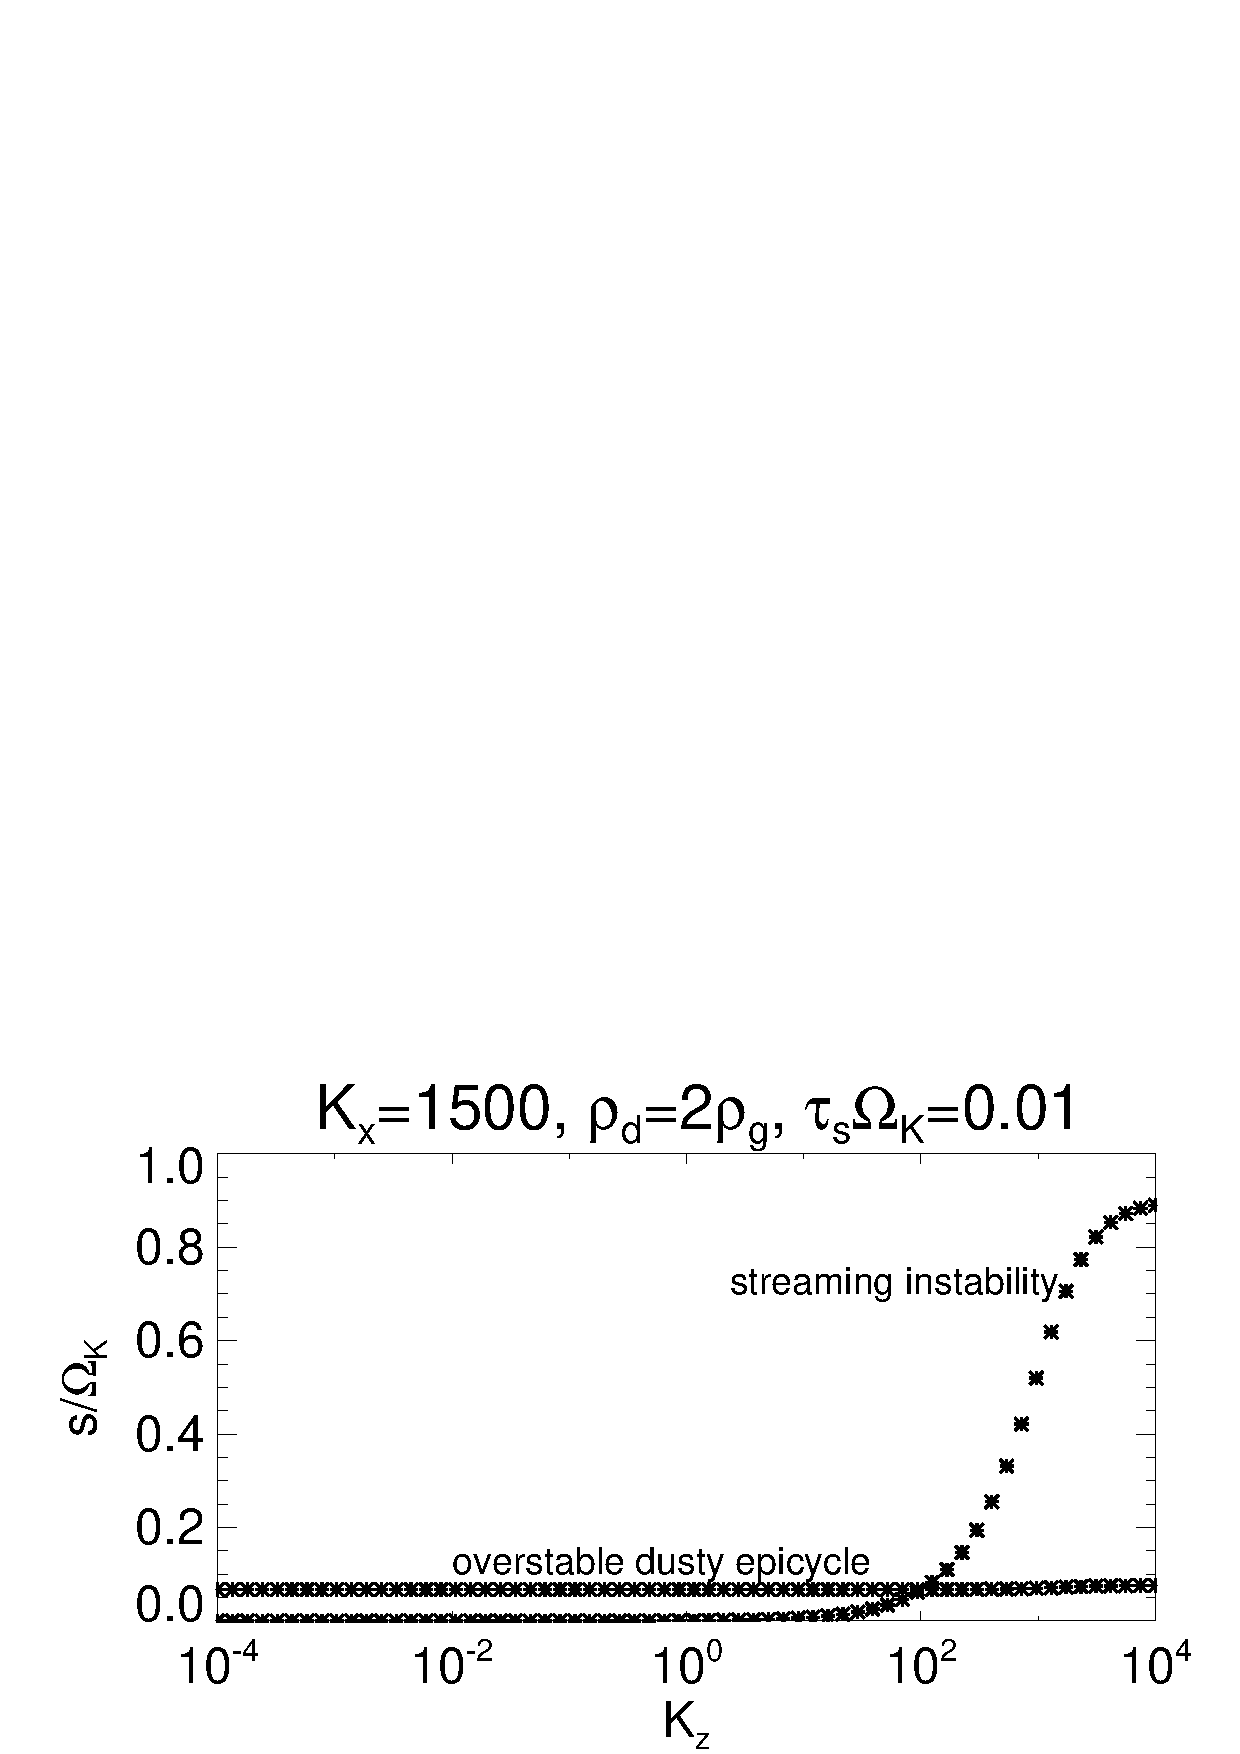
\includegraphics[width=\linewidth]{figures/streaming2}
  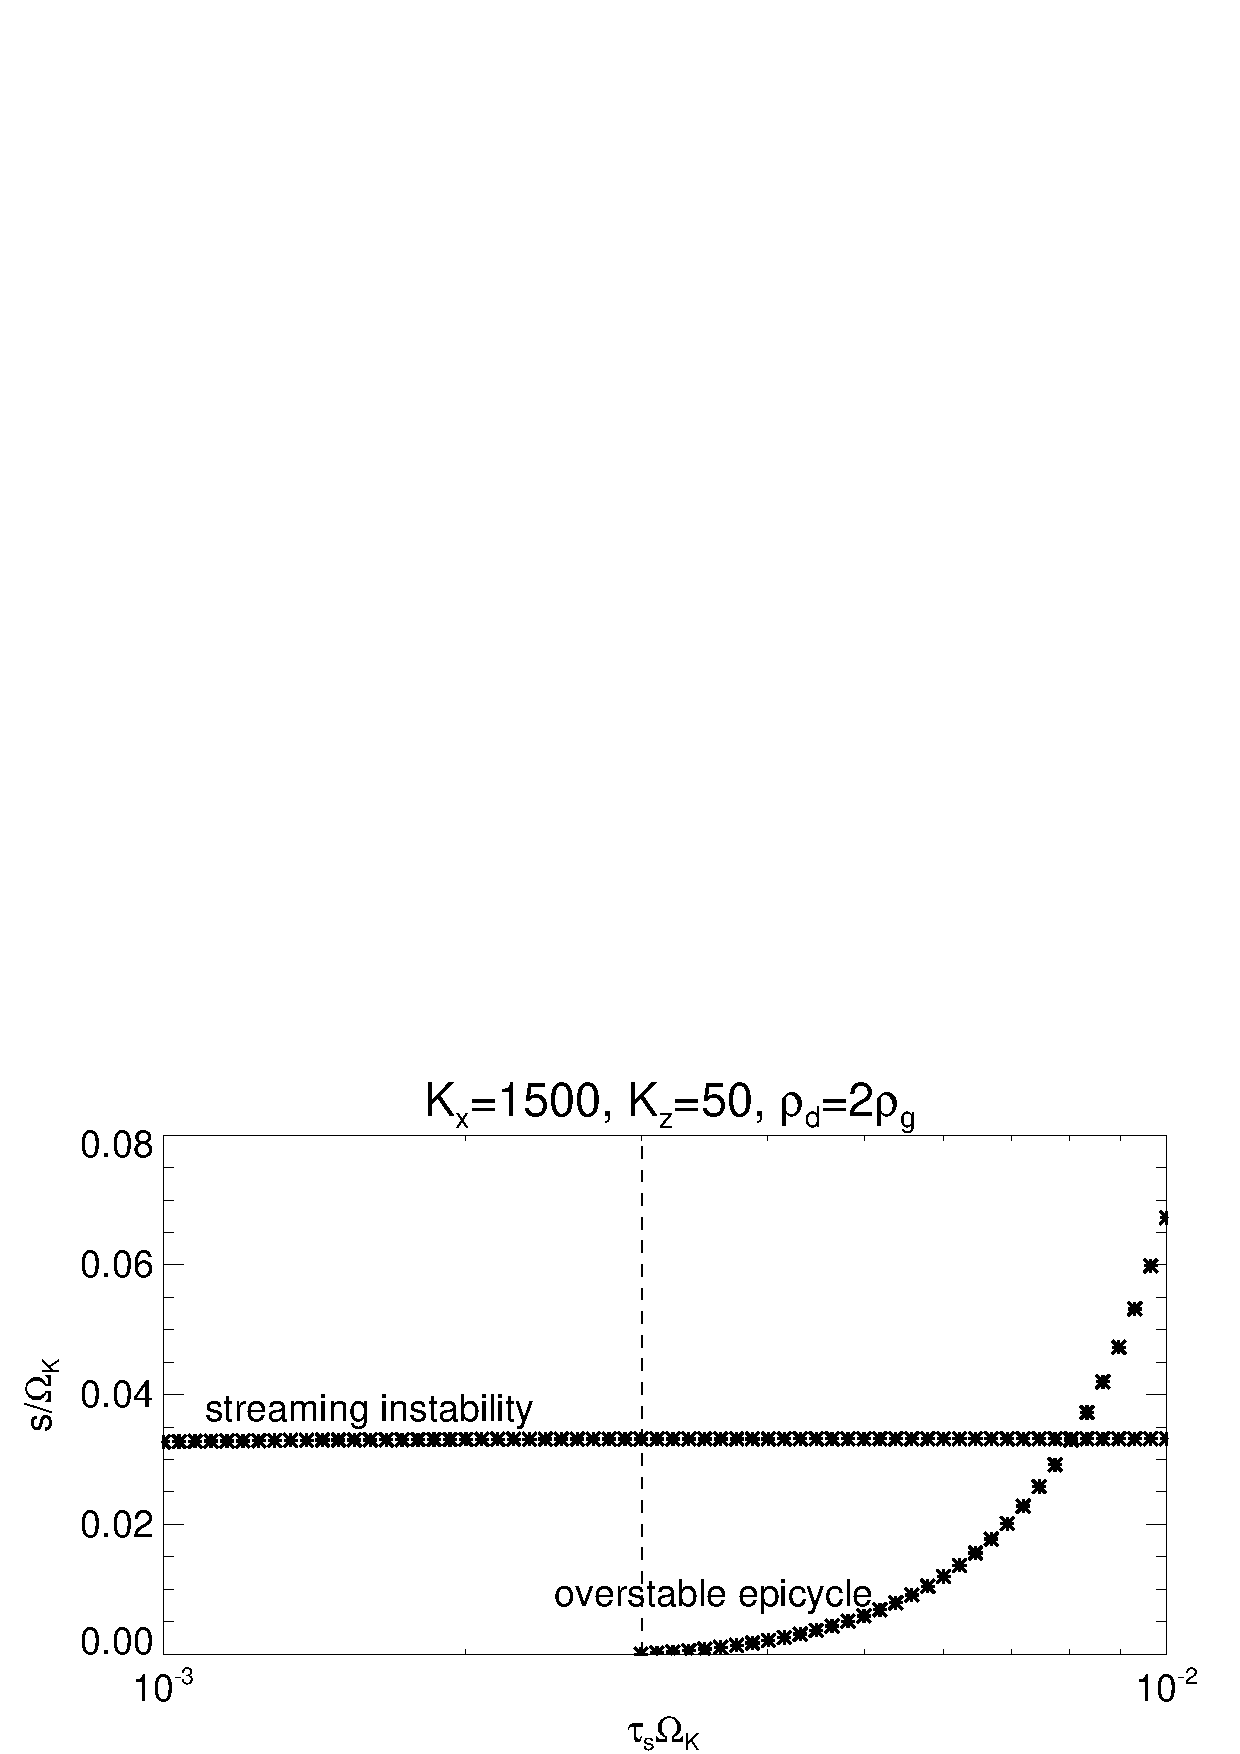
\includegraphics[width=\linewidth]{figures/streaming3}
  \caption{Growth rates of dust-drag instabilities with fixed radial
    wavenumber and dust-to-gas ratio, as a function of
    the vertical wavenumber at fix stopping time (top); and as a
    function of stopping time at fixed vertical wavenumber (bottom).  
\label{dusty_growth}
  }
\end{figure}


















%\subsection{Boundary conditions}
%Eq. \ref{lin_mass}---\ref{lin_energy} can be reduced to a set of
%first-order differential equations for $W, Q$ and $\dd v_z$. We can
%see this schematically as follows. Eq. \ref{lin_xmom} and
%\ref{lin_ymom} may be combined to yield 
%\begin{align*}
%  \dd v_r = \dd v_r (W, Q, \dd v_z). 
%\end{align*} 
%We can then take the continuity equation as an equation for $\dd v_z$, 
%\begin{align*}
%\text{Eq. \ref{lin_mass}} \Rightarrow \dd v_z^\prime(z) = \dd
%  v_z^\prime(W,Q,\dd v_z),
%\end{align*}
%and the vertical momentum equation as an equation for $Q$, 
%\begin{align*}
%\text{Eq. \ref{lin_zmom}} \Rightarrow Q^\prime(z) = 
% Q^\prime(W,Q,\dd v_z). 
%\end{align*}

%Now, for finite dust-gas coupling, $\tstop\neq0$, inspection of $\dd C$
%(Appendix \ref{lin_dust}) shows that it involves $W^\prime$ (assuming
%$\tepsilon < 1$). Then Eq. \ref{lin_energy} may be taken as a
%differential equation for $W$. However, for perfectly coupled dust,
%$\tstop =\dd\mathcal{C}= 0$. In that case Eq. \ref{lin_energy} gives an algebraic
%relation between $W$, $Q$ and $\dd v_z$. That is,
%\begin{align*}
%\text{Eq. \ref{lin_energy}}\Rightarrow \begin{cases}
%  W^\prime(z) = W^\prime(W, Q, \dd v_z) & \text{if } \tstop \neq 0, \\
%  W           (z) = W(Q, \dd v_z) & \text{if }\tstop = 0.
%\end{cases}
%\end{align*} 

%This means that for the perfectly coupled problem, we have a pair of
%ODEs for $Q$ and $\dd v_z$, and 
%When
%$\tstop\neq0$, we require three boundary conditions. {\bf WHAT?? Why odd
%  number of BCs? Shouldn't we have even number of BCs? We have
%two boundaries? I've only seen problems like this involving even
%number of BCs.} In this case we impose $\dd v_z =0$ at $z=\pm
%z_\mathrm{max}$, and classify modes according to their symmetry about
%the midplane: `even' modes with $\dd v_z^\prime(0) = 0$, and `odd' 
%modes with $\dd v_z(0)=0$.       

